\chapter{Conclusion and Future Work}

The goal of this thesis is to design paradigms and algorithms that enable individual cognitive radio to act autonomously, and finally converge to a equilibrium state, meanwhile, the performance of cognitive radio users are improved.
In this dissertation, we solve a series of problems residing from layer 1 to layer 3 in the OSI model~\cite{osi} of CRN with distributed solutions, and employ game theory to seek the guarantee on convergence and Nash equilibrium.
%Based on game models, we design distributed algorithms for CR users to self-organize and utilize the available resources, which doesn't lead to global instability or performance deterioration.

\section{Contribution}
We propose a complete strategy of power and spectrum allocation in IEEE 802.22 networks.
We make full use of the centralized database which is required by the standard and relevant regulations.
The maximal transmission power on channel for each WBS is decided in the database by solving an optimization problem.
Then a two stage channel power allocation scheme is proposed in a distributed manner, where the database is involved to assist interaction between secondary users.
This work lies in layer 1, after deciding the maximal transmission power on each secondary cellular base station, we formulate the distributed spectrum allocation problem in TV white space scenario (a special CRN where primary user is TV station which operates according to a slow and pre-decided schedule) into a canonical congestion game, then propose distributed algorithm corresponding to the behaviour of player in the game.

As to improving the accuracy of spectrum sensing with clusters, we designed a distributed clustering scheme ROSS.
ROSS is lightweight, thus is suitable CRAHN where the network connection varies due to the mobility of spectrum and secondary users.
ROSS increases the number of common available channels within one cluster, thus improves the robustness of formed clusters against primary users, so that cooperative sensing can make the best use of clusters.
%When the availability of spectrum is considered to have the same probability due to licensed users' activity, and local operation is needed, \ie for cooperative sensing, unlicensed users need to form clusters and the clusters should be robust against the primary users' activity.
%A distributed clustering scheme for CRN is proposed. 
%The process of finalizing cluster membership is innovatively formulated into a congestion game, then as long as cluster head is decided, clusters which have clear membership are formed quickly by applying the  light-weighted distributed scheme derived from the game.
This problem can be regarded to lie in layer 2.

In layer 3, we propose a lighted weighted routing scheme for CRN. 
Spectrum aware virtual coordinate is proposed, thus light weighted geographic routing can be used to decide the next hop.

\section{Future Work}
Building on the top of the our contributions, game theory can help to design distributed solution for further problems in CRN.
In this section, we describe the future work, and sketch the solutions briefly.
%Some further efforts can be done on the basis of the work in this thesis.

\subsection*{Structureless Diffusion Based Routing in Game Theoretical Framework in Event-driven Cognitive Radio Sensor Network}
One future work is to propose a structure less data fusion paradigm for cognitive radio sensor network.
Sensor nodes are deployed to sense physical phenomena of interests (PoIs), and they transmit the PoIs to the sink node.
Cognitive radio capability is transplanted onto sensor network~\cite{cr_sensor_2009}, so as to alleviate collision and decrease delay.
But congestion is still difficult to be totally eliminated by merely providing more spectrum.
%
Congestion occurs in wireless sensor network when incoming traffic load exceeds the capacity.
Variant solutions~\cite{congestion_control_wsn_2014} have been proposed to mitigate congestion, \eg implementing flow control to avoid transmitting to the downstream node where congestion is detected, changing the MAC behaviour to give the congested sensor larger possibility to transmit, adding rely nodes to reroute data around the congested nodes.


When there are multiple upstream nodes\footnote{Downstream nodes of one node $i$ represent the nodes relying data from node $i$ towards to the sink node, upstream nodes of node $i$ means the nodes sending data to node $i$.} transmitting to sink node, and there are several downstream nodes are available to be relies, then which portion of the data on the upstream node should be sent to which downstream node becomes a question.
As shown in Figure~\ref{futurework_1}, several nodes are downstream nodes for node 2 and 3.
%We look into the scenario where congestion happening on multiple downstream nodes, and we try to alleviate the congestion occurring at the run time by assigning the data of interests to suitable downstream nodes. 
We have proposed routing solution for end to end communication in CRN, where geographic routing is conducted with spectrum aware virtual coordinate.
As to multiple to one communication, simply using our proposed scheme is problematic, as we need to consider the possible collision caused by multiple transmission, priority of services and possible congestion appearing on the relying nodes.

\begin{figure}[h!]
  \centering
  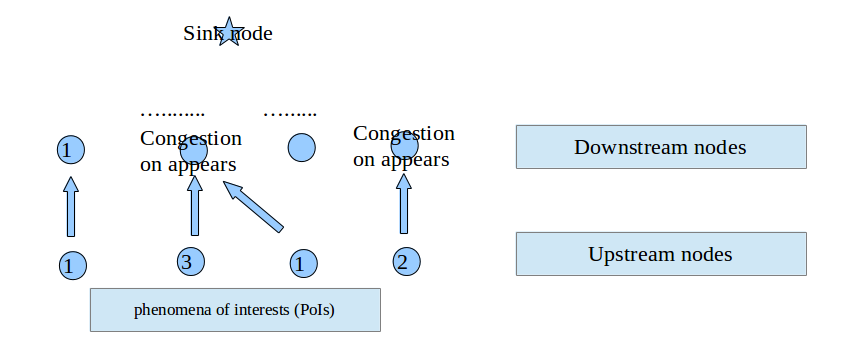
\includegraphics[width=0.8\linewidth]{futurework_1.png}
  \caption{Multiple to one communication}
  \label{futurework_1}
\end{figure}




\subsubsection*{Problem Statement}
The basic idea is from the \textit{server matching} introduced in Section~\ref{background}.
%As to a cognitive user, it passively receives data from upstream nodes, and then decides which portion of the data to be transmitted to which downstream node.

%chooses one downstream node whose congestion is increased smallest after accepting the data. Considering there could be multiple senders and receivers, such choosing strategy is not clear.


Delay of the packets is used to represent the congestion.
This delay could be the average of delay on all packets, or a function of delay of individual packet.
Although it is not clear how to granulate the data based on their priorities, it is clear that the total congestion (delay) is a increasing function of the amount of incoming data.
When there are only one group of downstream nodes and one group of upstream nodes involved, and the upstream nodes have finite number of transmission strategy (a certain portion is sent to a certain downstream node), then the convergence will be brought by best response strategy.
But the converge is not guaranteed when consider within a bigger picture, as the downstream nodes can  become upstream nodes when they send data to their downstream nodes.

The questions needed to be answered are as follows,
\begin{itemize}
\item What is the strategy for each sensor node to assign its data to different downstream nodes.
\item As this problem is a cascaded of congestion games, is there equilibrium?


\end{itemize}

 because the structured techniques incur relatively higher overheads to maintain the network structure. 





%Data can be aggregated if they are of the same attribute (and the same priority).
%The data with high priority demands small delay.


%\subsubsection{Scheme Sketch}
%
% This process is formulated into a player-specific singleton congestion game. Based on the property of this game model, data sender will finally decide on one downstream node using a heuristic greedy strategy, in other words, transmission topology will be formed swiftly.
%
%2. nodes send differentiated data to downstream nodes. The congestion function of node is decided by 
%\begin{itemize}
%\item 1. summation of inverted priorities of data after aggregation (in other words, there is no redundancy), 
%\item 2. workload of aggregating the data of the same attribute.
%\end{itemize}
%
%3. Function is ,  is the priority of the data of priority , is the effort of aggregating the data of the same attribute , is a parameter reflecting the normalized advanced distance from current node to this downstream node (need further considering), is a adjustment parameter. 
%
%4. Upstream nodes choose the downstream node whose congestion is increased smallest because of accepting its data, then upstream node sends out Decision Packet (note: this is not the payload packet but only one control single). Of course, this decision is open to change after other senders making decision, so there could be several rounds of Decision Packets transmissions.
%
%5. When the congestion resulted from the received decision packets is unchanged for a defined period of time, the node will notify its upstream nodes to send data to them. The same process of decision and transmission happens as step 2.
%
%-strong points and weak points
%1. strong points:
%1. structure less, no overhead for maintaining structure
%2. suitable for mobility
%3. Saving energy(aggregation decreases data to be sent)
%4. theoretical proof of quick decision on receiver
%2. weak points:
%1. Deciding on receiver incurs negotiation (signal exchange), overhead will be high when observed phenomena of interests is too frequent.
%
%This work can be extended to solve problems in sensor network, as long as change the congestion function.

\subsection*{Other Future Research Works}
\begin{itemize}
\item As to channel and power allocation in IEEE 802.22 network, cooperation can be brought to improve performance. 

\item As a light weight clustering scheme which can cope with mobility of both spectrum and users, ROSS can be used to support routing and resource allocation.
\end{itemize}




